% questions.tex —— 2006 年·普通高等学校招生考试·天津卷文科 · 题目内容片段（无答案）
% 由 tools/generate_projects.py 依来源总账自 2006/2006_数学真题_天津文_试题.md 生成，勿手改（改源 MD 后重跑）


\begin{gktip}
\textbf{来源边界}：题签依据固定候选 PDF 照录，题面为 PDF 第1—2页（印刷页码338—339）。固定副本的发布者、出版者、版次、来源链及官方身份未核；manifest 的 \texttt{ready} 仅表示文件状态，不代表来源认证。PDF 未见答案、解析或评分标准。
\end{gktip}

\gkpart{一、选择题}

\begin{question}
\gkti{1}已知集合 $A=\{x\mid -3\le x\le 1\}$，$B=\{x\mid |x|\le 2\}$，则 $A\cap B=$\mbox{（　　）}。

（A）$\{x\mid -2\le x\le 1\}$　　（B）$\{x\mid 0\le x\le 1\}$

（C）$\{x\mid -3\le x\le 2\}$　　（D）$\{x\mid 1\le x\le 2\}$

\end{question}
\begin{question}
\gkti{2}设 $\{a_n\}$ 是等差数列，$a_1+a_3+a_5=9$，$a_6=9$，则这个数列的前6项和等于\mbox{（　　）}。

（A）12　　（B）24　　（C）36　　（D）48

\end{question}
\begin{question}
\gkti{3}设变量 $x,y$ 满足约束条件
\nopagebreak[4]
\[
\begin{cases}y\le x,\\x+y\ge 2,\\y\ge 3x-6,\end{cases}
\]
则目标函数 $z=2x+y$ 的最小值为\mbox{（　　）}。

（A）2　　（B）3　　（C）4　　（D）9

\end{question}
\begin{question}
\gkti{4}设 $P=\log_2 3$，$Q=\log_3 2$，$R=\log_2(\log_3 2)$，则\mbox{（　　）}。

（A）$R<Q<P$　　（B）$P<R<Q$　　（C）$Q<R<P$　　（D）$R<P<Q$

\end{question}
\begin{question}
\gkti{5}设 $\alpha,\beta\in(-\frac\pi2,\frac\pi2)$，那么“$\alpha<\beta$”是“$\tan\alpha<\tan\beta$”的\mbox{（　　）}。

（A）充分而不必要条件　　（B）必要而不充分条件

（C）充分必要条件　　（D）既不充分也不必要条件

\end{question}
\begin{question}
\gkti{6}函数 $y=\sqrt{x^2+1}+1\ (x<0)$ 的反函数是\mbox{（　　）}。

（A）$y=\sqrt{x^2-2x}\ (x<0)$　　（B）$y=-\sqrt{x^2-2x}\ (x<0)$

（C）$y=\sqrt{x^2-2x}\ (x>2)$　　（D）$y=-\sqrt{x^2-2x}\ (x>2)$

\end{question}
\begin{question}
\gkti{7}若 $l$ 为一条直线，$\alpha,\beta,\gamma$ 为三个互不重合的平面，给出下面三个命题：

① $\alpha\perp\gamma,\ \beta\perp\gamma\Rightarrow\alpha\perp\beta$；

② $\alpha\perp\gamma,\ \beta\parallel\gamma\Rightarrow\alpha\perp\beta$；

③ $l\parallel\alpha,\ l\perp\beta\Rightarrow\alpha\perp\beta$。

其中正确的命题有\mbox{（　　）}。

（A）0个　　（B）1个　　（C）2个　　（D）3个

\end{question}
\begin{question}
\gkti{8}椭圆的中心为点 $E(-1,0)$，它的一个焦点为 $F(-3,0)$，相应于焦点 $F$ 的准线方程为 $x=-\frac72$，则这个椭圆的方程是\mbox{（　　）}。

（A）$\frac{2(x-1)^2}{21}+\frac{2y^2}{3}=1$　　（B）$\frac{2(x+1)^2}{21}+\frac{2y^2}{3}=1$

（C）$\frac{(x-1)^2}{5}+y^2=1$　　（D）$\frac{(x+1)^2}{5}+y^2=1$

\end{question}
\begin{question}
\gkti{9}已知函数 $f(x)=a\sin x-b\cos x$（$a\text{、}b$为常数，$a\ne0\text{，}x\in\mathbb R$）的图象关于直线 $x=\frac\pi4$ 对称，则函数 $y=f(\frac{3\pi}4-x)$ 是\mbox{（　　）}。

（A）偶函数且图象关于点 $(\pi,0)$ 对称

（B）偶函数且图象关于点 $(\frac{3\pi}2,0)$ 对称

（C）奇函数且图象关于点 $(\frac{3\pi}2,0)$ 对称

（D）奇函数且图象关于点 $(\pi,0)$ 对称

\end{question}
\begin{question}
\gkti{10}如果函数 $f(x)=a^x(a^x-3a^2-1)$（$a>0$且$a\ne1$）在区间 $[0,+\infty)$ 上是增函数，那么实数 $a$ 的取值范围是\mbox{（　　）}。

（A）$(0,\frac23]$　　（B）$[\frac{\sqrt3}3,1)$　　（C）$(1,\sqrt3]$　　（D）$[\frac32,+\infty)$

\end{question}
\gkpart{二、填空题}

\begin{question}
\gkti{11}$(x+\frac1{\sqrt{x}})^7$ 的二项展开式中 $x$ 的系数是\gkblank{}。（用数字作答）

\end{question}
\begin{question}
\gkti{12}设向量 $\boldsymbol a$ 与 $\boldsymbol b$ 的夹角为 $\theta$，且 $\boldsymbol a=(3,3)$，$2\boldsymbol b-\boldsymbol a=(-1,1)$，则 $\cos\theta=$\gkblank{}。

\Needspace{0.4\textheight}
\end{question}
\begin{question}
\gkti{13}如图，在正三棱柱 $ABC-A_1B_1C_1$ 中，$AB=1$。若二面角 $C-AB-C_1$ 的大小为 $60^\circ$，则点 $C$ 到平面 $ABC_1$ 的距离为\gkblank{}。
\nopagebreak[4]
\begin{center}% 2006 天津文科 Q13，源：固定 PDF 第 1 页（印刷页 338）。
% 识别映射：实棱 AB, BC, AA_1, BB_1, CC_1, A_1B_1, B_1C_1, C_1A_1, BC_1；
% 虚棱 AC；虚线段 AC_1。节点为 A,B,C,A_1,B_1,C_1。原图中 AC 与 AC_1 均为虚线。
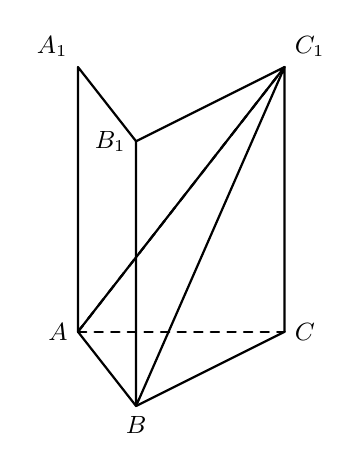
\begin{tikzpicture}[x=0.82cm,y=0.82cm,line cap=round,line join=round,line width=0.8pt,font=\small]
  \coordinate (A) at (0,0);
  \coordinate (B) at (0.9,-1.15);
  \coordinate (C) at (3.2,0);
  \coordinate (A1) at (0,4.1);
  \coordinate (B1) at (0.9,2.95);
  \coordinate (C1) at (3.2,4.1);
  \draw[dashed] (A)--(C);
  \draw[dashed] (A)--(C1);
  \draw (A)--(B)--(C);
  \draw (A)--(A1)--(B1)--(C1)--cycle;
  \draw (B)--(B1) (C)--(C1) (B)--(C1);
  \node[left] at (A) {$A$};
  \node[below] at (B) {$B$};
  \node[right] at (C) {$C$};
  \node[above left] at (A1) {$A_1$};
  \node[left] at (B1) {$B_1$};
  \node[above right] at (C1) {$C_1$};
\end{tikzpicture}
\end{center}
\nopagebreak[4]
\end{question}
\begin{question}
\gkti{14}若半径为1的圆分别与 $y$ 轴的正半轴和射线 $y=\frac{\sqrt3}{3}x\ (x\ge0)$ 相切，则这两个圆的方程为\gkblank{}。

\end{question}
\begin{question}
\gkti{15}某公司一年购买某种货物400吨，每次都购买 $x$ 吨，运费为4万元/次，一年的总存储费用为 $4x$ 万元，要使一年的总运费与总存储费用之和最小，则 $x=$\gkblank{}吨。

\end{question}
\begin{question}
\gkti{16}用数字0、1、2、3、4组成没有重复数字的五位数，则其中数字1、2相邻的偶数有\gkblank{}个。（用数字作答）

\end{question}
\gkpart{三、解答题}

\begin{question}
\gkti{17}已知 $\tan\alpha+\cot\alpha=\frac52$，$\alpha\in(\frac\pi4,\frac\pi2)$，求 $\cos2\alpha$ 和 $\sin(2\alpha+\frac\pi4)$ 的值。

\end{question}
\begin{question}
\gkti{18}甲、乙两台机床相互没有影响地生产某种产品，甲机床产品的正品率是0.9，乙机床产品的正品率是0.95。

（1） 从甲机床生产的产品中任取3件，求其中恰有2件正品的概率（用数字作答）；

（2） 从甲、乙两台机床生产的产品中各任取1件，求其中至少有1件正品的概率（用数字作答）。

\Needspace{0.4\textheight}
\end{question}
\begin{question}
\gkti{19}如图，在五面体 $ABCDEF$ 中，点 $O$ 是矩形 $ABCD$ 的对角线的交点，面 $CDE$ 是等边三角形，棱 $EF\parallel BC$ 且 $EF=\frac12BC$。

（1） 证明：$FO\parallel$ 平面 $CDE$；

（2） 设 $BC=\sqrt3CD$，证明：$EO\perp$ 平面 $CDF$。
\nopagebreak[4]
\begin{center}% 2006 天津文科 Q19，源：固定 PDF 第 1 页（印刷页 338）。
% 节点：A,B,C,D 为矩形 ABCD 的角点，O 为对角线交点；E,F 为等边三角形 CDE
% 的第三顶点与棱端点。识别的实线：BC, CD, DE, EF, FB, EC, FC。
% 识别的虚线：AB, AD, AF, FO, EO, FD。题干说 O 是矩形 ABCD 对角线交点，
% 但源图未画 AC/BD 对角线，故未补画；O 是 FO 与 EO 两条虚线的端点。
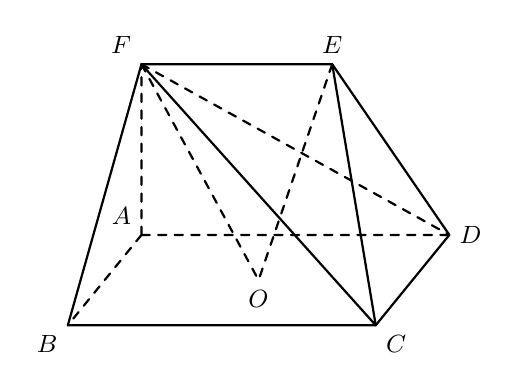
\begin{tikzpicture}[x=0.85cm,y=0.85cm,line cap=round,line join=round,line width=0.8pt,font=\small]
  \coordinate (A) at (1.1,1.35);
  \coordinate (B) at (0,0);
  \coordinate (C) at (4.6,0);
  \coordinate (D) at (5.7,1.35);
  \coordinate (O) at (2.85,0.675);
  \coordinate (F) at (1.1,3.9);
  \coordinate (E) at (3.95,3.9);
  % 隐藏棱与辅助虚线
  \draw[dashed] (A)--(B) (A)--(D) (A)--(F);
  \draw[dashed] (F)--(O) (E)--(O) (F)--(D);
  % 可见棱及内部实线
  \draw (B)--(C)--(D)--(E)--(F)--(B);
  \draw (E)--(C) (F)--(C);
  \node[above left] at (A) {$A$};
  \node[below left] at (B) {$B$};
  \node[below right] at (C) {$C$};
  \node[right] at (D) {$D$};
  \node[above] at (E) {$E$};
  \node[above left] at (F) {$F$};
  \node[below] at (O) {$O$};
\end{tikzpicture}
\end{center}
\nopagebreak[4]
\end{question}
\begin{question}
\gkti{20}已知函数 $f(x)=4x^3-3x^2\cos\theta+\frac1{32}$，其中 $x\in\mathbb R$，$\theta$ 为参数，且 $0\le\theta\le\frac\pi2$。

（1） 当 $\cos\theta=0$ 时，判断函数 $f(x)$ 是否有极值；

（2） 要使函数 $f(x)$ 的极小值大于零，求参数 $\theta$ 的取值范围；

（3） 若对（2） 中所求的取值范围内的任意参数 $\theta$，函数 $f(x)$ 在区间 $(2a-1,a)$ 内都是增函数，求实数 $a$ 的取值范围。

\end{question}
\begin{question}
\gkti{21}已知数列 $\{x_n\}$ 满足 $x_1=x_2=1$，并且
\nopagebreak[4]
\[
\frac{x_{n+1}}{x_n}=\lambda\frac{x_n}{x_{n-1}}\quad(\lambda\text{为非零参数},\ n=2,3,4,\cdots)
\]

（1） 若 $x_1,x_3,x_5$ 成等比数列，求参数 $\lambda$ 的值；

\Needspace{5\baselineskip}
（2） 设 $0<\lambda<1$，常数 $k\in\mathbb N^*$ 且 $k\ge3$，证明：
\nopagebreak[4]
\[
\frac{x_{1+k}}{x_1}+\frac{x_{2+k}}{x_2}+\cdots+\frac{x_{n+k}}{x_n}<\frac{\lambda^k}{1-\lambda^k}\quad(n\in\mathbb N^*)
\]

\Needspace{0.4\textheight}
\end{question}
\begin{question}
\gkti{22}如图，双曲线 $\frac{x^2}{a^2}-\frac{y^2}{b^2}=1\ (a>0,b>0)$ 的离心率为 $\frac{\sqrt5}2$，$F_1,F_2$ 分别为左、右焦点，$M$ 为左准线与渐近线在第二象限内的交点，且 $\overrightarrow{F_1M}\cdot\overrightarrow{F_2M}=-\frac14$。

（1） 求双曲线的方程；

（2） 设 $A(m,0)$ 和 $B(\frac1m,0)\ (0<m<1)$ 是 $x$ 轴上的两点。过点 $A$ 作斜率不为0的直线 $l$，使得 $l$ 交双曲线于 $C,D$ 两点，作直线 $BC$ 交双曲线于另一点 $E$。证明：直线 $DE$ 垂直于 $x$ 轴。
\nopagebreak[4]
\begin{center}% 2006 天津文科 Q22，源：固定 PDF 第 2 页（印刷页 339）。
% 几何比例依题面推出的 x^2-4y^2=1 作示意；以 m=3/4、参数 p=1/10 为一组
% 可行示例定位 A,B,C,D,E。拓扑：渐近线过 O；左准线过 M；DE 竖直；l 为 D-A-C，
% BC 为 E-C-B。其余焦点位置按 F1,F2=(±sqrt(5)/2,0)。
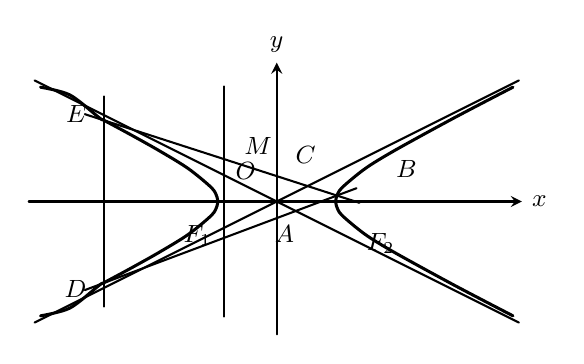
\begin{tikzpicture}[x=0.75cm,y=0.75cm,line cap=round,line join=round,line width=0.75pt,font=\small,>=stealth]
  % 坐标轴
  \draw[->] (-4.2,0)--(4.15,0) node[right] {$x$};
  \draw[->] (0,-2.25)--(0,2.35) node[above] {$y$};

  % 左准线 x=-2/sqrt(5)，及同一竖直线上的 D、E
  \draw (-0.894,-1.95)--(-0.894,1.95);
  \draw (-2.922,-1.78)--(-2.922,1.78);

  % 双曲线 x^2-4y^2=1
  \draw[line width=1.1pt] plot[smooth] coordinates {
    (-4,1.936) (-3.5,1.803) (-3,1.414) (-2.922,1.373)
    (-2.5,1.146) (-2,0.866) (-1.5,0.559) (-1.1,0.229)
    (-1.01,0.071) (-1,0)
  };
  \draw[line width=1.1pt] plot[smooth] coordinates {
    (-4,-1.936) (-3.5,-1.803) (-3,-1.414) (-2.922,-1.373)
    (-2.5,-1.146) (-2,-0.866) (-1.5,-0.559) (-1.1,-0.229)
    (-1.01,-0.071) (-1,0)
  };
  \draw[line width=1.1pt] plot[smooth] coordinates {
    (1,0) (1.01,0.071) (1.1,0.229) (1.5,0.559)
    (2,0.866) (3,1.414) (4,1.936)
  };
  \draw[line width=1.1pt] plot[smooth] coordinates {
    (1,0) (1.01,-0.071) (1.1,-0.229) (1.5,-0.559)
    (2,-0.866) (3,-1.414) (4,-1.936)
  };

  % 渐近线，以及 l=D-A-C、BC=E-C-B
  \draw (-4.1,2.05)--(4.1,-2.05);
  \draw (-4.1,-2.05)--(4.1,2.05);
  \draw (-3.25,-1.5)--(1.35,0.225);
  \draw (-3.25,1.479)--(1.4,-0.022);

  % 关键点（示意参数 m=3/4,p=1/10）
  \node[left] at (-3.05,1.48) {$E$};
  \node[left] at (-3.05,-1.48) {$D$};
  \node[above right] at (-0.72,0.62) {$M$};
  \node[below] at (-1.34,-0.24) {$F_1$};
  \node[above left] at (-0.18,0.20) {$O$};
  \node[below left,xshift=-6pt,yshift=-5pt] at (0.75,0) {$A$};
  \node[above left,xshift=-4pt,yshift=8pt] at (1.02,0.101) {$C$};
  \node[below right,xshift=5pt,yshift=-8pt] at (1.118,0) {$F_2$};
  \node[above right,xshift=11pt,yshift=5pt] at (1.333,0) {$B$};
\end{tikzpicture}
\end{center}
\nopagebreak[4]

\end{question}